\section{Introduction}
\begin{figure}[htbp]
    \centering
    \includegraphics[width=1.0\linewidth]{figures/figure_gate.png}
    \caption{\textbf{Agile flight through narrow gates.} (\textbf{A}) Caltech Real Weather Wind Tunnel system, the quadrotor UAV, and the gate. In our flight tests, the UAV follows an agile trajectory through narrow gates, which are slightly wider than the UAV itself, under challenging wind conditions. (\textbf{B-C}) Trajectories used for the gate tests. In (B), the UAV follows a figure-8 through one gate, with wind speed \SI{3.1}{m/s} or time-varying wind condition. In (C), the UAV follows an ellipse in the horizontal plane through two gates, with wind speed \SI{3.1}{m/s}. (\textbf{D-E}) Long-exposure photos (with an exposure time of \SI{5}{s}) showing one lap in two tasks. (\textbf{F-I}) High-speed photos (with a shutter speed of 1/200\SI{}{s}) showing the moment the UAV passed through the gate and the interaction between the UAV and the wind.}
    \label{fig:intro}
\end{figure}

% Problem - precise flight control
The commoditization of uninhabited aerial vehicles (UAVs) \revB{requires that the control of these vehicles become more precise and agile}. For example, drone delivery requires transporting goods to a narrow target area in various weather conditions; drone rescue and search require entering and searching collapsed buildings with little space; urban air mobility needs a flying car to follow a planned trajectory closely to avoid collision in the presence of strong unpredictable winds.

% Challenge of unmodeled aerodynamics; difficulty of modeling approaches; motivate data driven approach
Unmodeled and often complex aerodynamics are among the most \revB{notable} challenges to precise flight control. 
Flying in windy environments (as shown in \cref{fig:intro}) introduces even more complexity because of the unsteady aerodynamic interactions between the drone, the induced airflow, and the wind (see \cref{fig:intro}(F) for a smoke visualization). These unsteady and nonlinear aerodynamic effects substantially degrade the performance of conventional UAV control methods that neglect to account for them in the control design. Prior approaches partially capture these effects with simple linear or quadratic air drag models, which limit the tracking performance in agile flight and cannot be extended to external wind conditions \cite{foehn2021time,faessler_differential_2018}. 
Although more complex aerodynamic models can be derived from computational fluid dynamics \cite{ventura2018high}, such modelling is often computationally expensive, and is limited to steady non-dynamic wind conditions. \rev{Adaptive control addresses this problem by estimating linear parametric uncertainty in the dynamical model in real time to improve tracking performance. Recent \sota~in quadrotor flight control has used adaptive control methods that directly 
% There has been recent popularity and success using adaptive control methods which directly 
estimate the unknown aerodynamic force without assuming the structure of the underlying physics, but relying on high-frequency and low-latency control \cite{tal_accurate_2021,mallikarjunan_l1_2012,pravitra_L1-adaptive_2020,hanover_performance_2021}.}
In parallel, there has been increased interest in data-driven modeling of aerodynamics (e.g., \cite{shi2019neural,shi2020neural,shi2021neural,torrente2021data}),
%Recently, data-driven modelling for aerodynamic disturbance has caught attention. For example, in previous work, we developed learning-based controllers in presence of fixed disturbances, such as the ground effect when a drone is close to the ground \cite{shi2019neural} and the downwash effect when a drone is below another vehicle \cite{shi2020neural,shi2021neural}. 
%Similarly, \cite{torrente2021data} uses Gaussian Processes to learn aerodynamic effects offline using precollected data. However, \cite{shi2019neural,shi2020neural,shi2021neural,torrente2021data} 
however existing approaches cannot effectively adapt in changing or unknown environments such as time-varying wind conditions.

% \subsection*{Overview of \nf~and Significance}
In this \revB{article}, we present a data-driven approach called \nf, which is a deep-learning-based trajectory tracking controller that learns to quickly adapt to rapidly-changing wind conditions. 
Our method, depicted in \cref{fig:block-diagram}, advances and offers insights into both adaptive flight control and deep-learning-based robot control.
% Our framework allows for an efficient but rich representation of unmodeled dynamics to be trained offline then quickly adapted online with formal stability guarantees. 
Our experimental demonstrates that \nf~achieves centimeter-level position-error tracking of an agile and challenging trajectory in dynamic wind conditions on a \rev{standard} UAV.

% overview of offline learning phase
Our method has two main components: an offline learning phase and an online adaptive control phase used as real-time online learning. For the offline learning phase, we have developed \LearningAlg~(\DAML) that learns a wind-condition-independent deep neural network (DNN) representation of the aerodynamics in a data-efficient manner. 
The output of the DNN is treated as a set of basis functions that represent the aerodynamic effects. This representation is adapted to different wind conditions by updating a set of linear coefficients that mix the output of the DNN. 
\DAML~\rev{is data efficient and} uses only 12 total minutes of flight data in \rev{just} 6 different wind conditions to train the DNN. 
% Second, in the online control phase, only the 12 linear coefficients mixing the output of the DNN are adapted to a new wind condition.
% Such data efficiency is a direct result of our unified approach and algorithm design.
\DAML~incorporates several key features which not only improve the data efficiency but also are informed by the downstream online adaptive control phase. In particular, \DAML~uses spectral normalization \cite{shi2019neural,bartlett2017spectrally} to control the Lipschitz property of the DNN to improve generalization to unseen data and \rev{provide closed-loop stability and robustness guarantees.} \DAML~also uses a discriminative network, which ensures that the learned representation is wind-\rev{invariant} and that the wind-dependent information is only contained in the linear coefficients that are adapted in the online control phase.

% overview of online control phase
For the online adaptive control phase, we have developed a regularized composite adaptive control law, which \rev{we} derived from a fundamental understanding of how the learned representation interacts with the closed-loop control system and which \rev{we} support \rev{with} rigorous theory. The use of composite adaptive control was inspired by~\cite{slotine1991applied,slotine_composite_1989}. The adaptation law updates the wind-dependent linear coefficients using a composite of the position tracking error term and the aerodynamic force prediction error term. Such a principled approach effectively guarantees stable and fast adaptation to any wind condition and robustness against imperfect learning. \rev{Although this adaptive control law could be used with a number of learned models,} the speed of adaptation is further aided by the concise representation learned from \DAML.
% Moreover, we incorporate a regularization term for rigorous stability guarantees and robustness to quickly changing wind conditions. 

\begin{figure}[htbp]
    \centering
    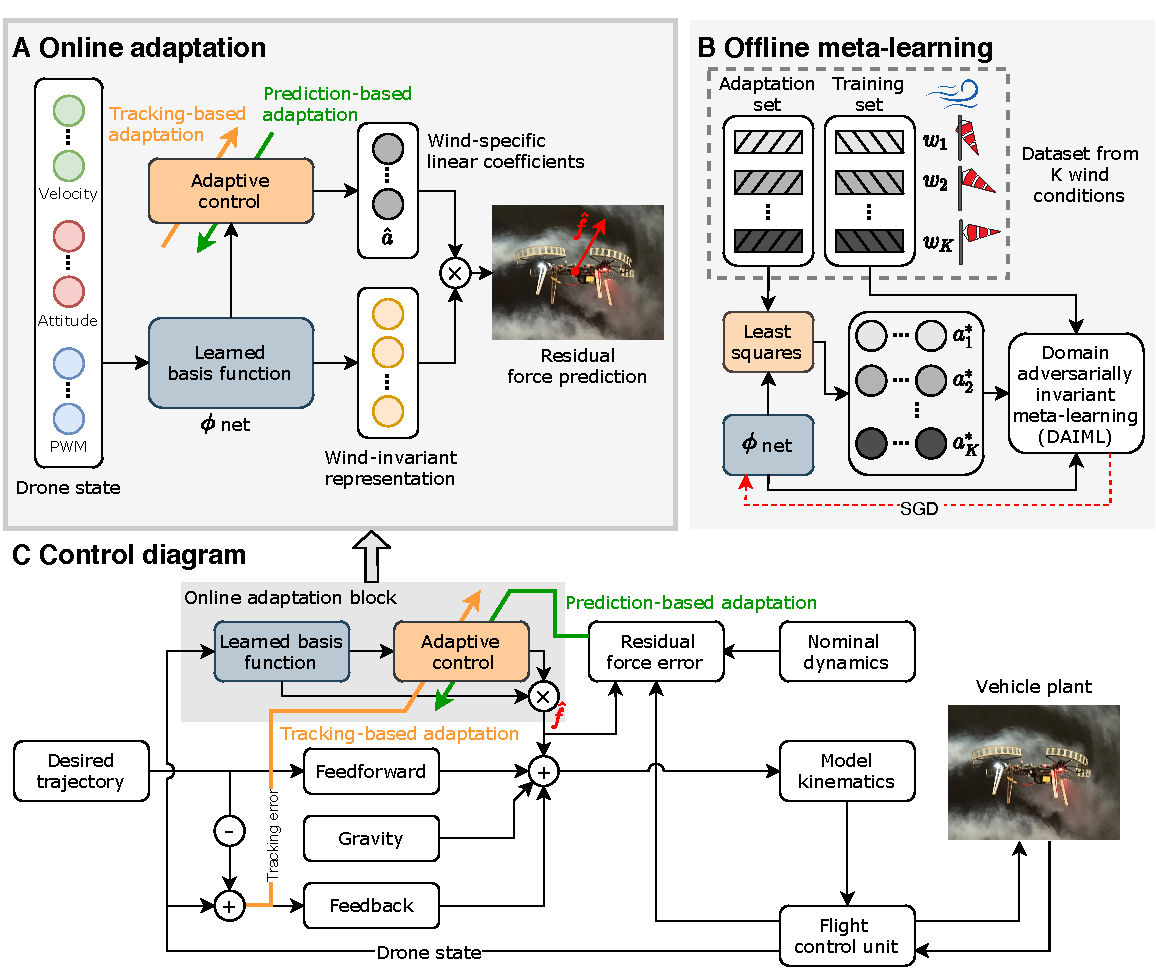
\includegraphics[width=1.0\linewidth]{figures/figure_learning_diagram.pdf}
    \caption{\textbf{Offline meta-learning and online adaptive control design.} (\textbf{A}) The online adaptation block in our adaptive controller. Our controller leverages the meta-trained basis function $\phi$, which is a wind-invariant representation of the aerodynamic effects, and uses composite adaptation (that is, including tracking-error-based and prediction-error-based adaptation) to update wind-specific linear weights $\hat{a}$. The output of this block is the wind-effect force estimate, $\hat{f}=\phi\hat{a}$. (\textbf{B}) The illustration of our meta-learning algorithm \DAML. We collected data from wind conditions $\{w_1,\cdots,w_K\}$ and applied Algorithm \ref{alg:DIML} to train the $\phi$ net. (\textbf{C}) The diagram of our control method, where the grey part corresponds to (A). Interpreting the learned block as an aerodynamic force allows it to be incorporated into the feedback control easily.}
    \label{fig:block-diagram}
\end{figure}

% Summary of key results
% With our method \nf, we report an order of magnitude improvement in the tracking performance over a conventional PID controller (similar to the built-in PX4 method) and a greater than two-fold improvement over both a state-of-the-art nonlinear tracking controller and a disturbance-observing adaptive controller.
\rev{Using \nf, we report an average improvement of \SI{66}{\%} over a nonlinear tracking controller, \SI{42}{\%} over an $\LOne$ adaptive controller, and \SI{35}{\%} over an Incremental Nonlinear Dynamics Inversion (INDI) controller.}
These results are all accomplished using standard quadrotor UAV hardware, while running the PX4's default regulation attitude control. Our tracking performance is competitive even compared to related work without external wind disturbances and with more complex hardware (for example, \cite{tal_accurate_2021} requires a 10-time higher control frequency and onboard optical sensors for direct motor speed feedback). 
\rev{We also compare \nf~with two variants of our method: \nftransfer, which uses a learned representation trained on data from a different drone, and \nfconstant, which only uses our adaptive control law with a trivial non-learning basis.
\nftransfer~demonstrates that our method is robust to changes in vehicle configuration and model mismatch. \nfconstant, $\LOne$, and INDI all directly adapt to the unknown dynamics without assuming the structure of the underlying physics, and they have similar performance.}
Furthermore, we demonstrate that our method enables a new set of capabilities that allow the UAV to fly through low-clearance gates following agile trajectories in gusty wind conditions (\cref{fig:intro}).

% Related work

\rev{\subsection*{Related Work for Precise Quadrotor Control}}
\rev{
Typical quadrotor control consists of a cascaded or hierarchical control structure which separates the design of the position controller, attitude controller, and thrust mixer (allocation). Commonly-used off-the-shelf controllers, such as PX4, design each of these loops as proportional-integral-derivative (PID) regulation controllers \cite{meier_pixhawk_2012}. The control performance can be substantially improved by designing each layer of the cascaded controller as a tracking controller using the concept of differential flatness \cite{mellinger_minimum_2011}, or, as has recently been popular, using a single optimization based controller such as model predictive control (MPC) to directly compute motor speed commands from desired trajectories. State-of-the-art tracking performance relies on MPC with fast adaptive inner loops to correct for modeling errors \cite{tal_accurate_2021,hanover_performance_2021}, however, this approach requires full custom flight controllers. In contrast, our method is designed to be integrated with a typical PX4 flight controller, yet it achieves state-of-the-art flight performance in wind.
% First we introduce related work on agile quadrotor control without wind disturbances. Even flying in the free space without external wind, agile quadrotor control requires non-trivial design as there are substantial aerodynamic effects such as air drag not considered by standard controllers \cite{foehn2021time,tal_accurate_2021}. Quadrotor control, as part of multicopter control, generally has a cascaded structure to separate the design of the position controller, attitude controller, and thrust mixer (allocation). Commonly-used off-the-shelf controllers, such as PX4, design each of these loops as regulation controllers \cite{meier_pixhawk_2012}, which perform well in gentle tasks but become unsatisfactory for agile flights. Therefore tracking controllers are developed, which have a similar cascaded structure to the regulation controllers, but use the concept of differential flatness to derive desired angular rates and accelerations for the attitude control directly from the position trajectory \cite{mellinger_minimum_2011}.
}

\rev{
Prior work on agile quadrotor control has achieved impressive results by considering aerodynamics~\cite{tal_accurate_2021,hanover_performance_2021,torrente2021data,faessler_differential_2018}. However, those approaches require specialized onboard hardware~\cite{tal_accurate_2021}, full custom flight control stacks~\cite{tal_accurate_2021,hanover_performance_2021}, or cannot adapt to external wind disturbances~\cite{torrente2021data,faessler_differential_2018}.
For example, state-of-the-art tracking performance has been demonstrated using incremental nonlinear dynamics inversion to estimate aerodynamic disturbance forces, with a root-mean-square tracking error of \SI{6.6}{cm} and drone ground speeds up to \SI{12.9}{m/s} \cite{tal_accurate_2021}. However, \cite{tal_accurate_2021} relies on high-frequency control updates (\SI{500}{Hz}) and direct motor speed feedback using optical encoders to rapidly estimate external disturbances. Both are challenging to deploy on standard systems. 
\cite{hanover_performance_2021} simplifies the hardware setup and does not require optical motor speed sensors and has demonstrated state-of-the-art tracking performance. However, \cite{hanover_performance_2021} relies on a high-rate $\LOne$ adaptive controller inside a model predictive controller and uses a racing drone with a fully customized control stack.
\cite{torrente2021data} leverages an aerodynamic model learned offline and represented as Gaussian Processes. % to achieve a  root-mean-square tracking error down to \SI{15}{cm} during tests with similar ground speeds as our experiments. 
However, \cite{torrente2021data} cannot adapt to unknown or changing wind conditions and provides no theoretical guarantees. Another recent work focuses on deriving simplified rotor-drag models that are differentially flat \cite{faessler_differential_2018}. 
However, \cite{faessler_differential_2018} focuses on horizontal, $xy-$plane trajectories at ground speeds of \SI{4}{m/s} without external wind, where the thrust is more constant than ours, achieves $\sim$\SI{6}{cm} tracking error \cite{faessler_differential_2018}, uses an attitude controller running at \SI{4000}{Hz}, and is not extensible to faster flights as pointed out in \cite{torrente2021data}.
% More details on how our hardware and method compare to other state-of-the-art works in quadrotor flight control are provided in the supplementary material (\ref{sec:supp-drone-configuration})
}\\

\subsection*{Relation between \nf~and Conventional Adaptive Control}
% introduce adaptive control and main challenges with it
Adaptive control theory has been extensively studied for online control and identification problems with parametric uncertainty, for example, unknown linear coefficients for mixing known basis functions \cite{slotine1991applied,ioannou1996robust,krstic1995nonlinear,narendra2012stable,farrell_adaptive_2006,wise2006adaptive}. There are three common aspects of adaptive control which must be addressed carefully in any well-designed system and which we address in \nf: designing suitable basis functions for online adaptation, stability of the closed-loop system, and persistence of excitation, which is a property related to robustness against disturbances. \revB{These challenges arise due to the coupling between the unknown underlying dynamics and the online adaptation.
This coupling precludes naive combinations of online learning and control. For example, gradient-based parameter adaptation has well-known stability and robustness issues as discussed in \cite{slotine1991applied}. The idea of composite adaptation was first introduced in~\cite{slotine_composite_1989}.
}

% Challenge of designing basis functions
The basis functions play a crucial role in the performance of adaptive control, but designing or selecting proper basis functions might be challenging. A good set of basis functions should reflect important features of the underlying physics. In practice, basis functions are often designed using physics-informed modeling of the system, such as the nonlinear aerodynamic modeling in \cite{shi_adaptive_2020}. However, physics-informed modeling requires a tremendous amount of prior knowledge and human labor, and is often still inaccurate. Another approach is to use random features as the basis set, such as random Fourier features \rev{ \cite{rahimi2007random,lale_model_2021}}, which can model all possible underlying physics as long as the number of features is large enough. However, the high-dimensional feature space is not optimal for a specific system because many of the features might be redundant or irrelevant. Such suboptimality and redundancy not only increase the computational burden but also slow down the convergence speed of the adaptation process.

% Stability and p.e. challenges of adaptive control 
Given a set of basis functions, naive adaptive control designs may cause instability and fragility in the closed-loop system, due to the nontrivial coupling between the adapted model and the system dynamics. 
In particular, asymptotically stable adaptive control cannot guarantee robustness against disturbances and so exponential stability is desired.  Even so, often, existing adaptive control methods only guarantee exponential stability when the desired trajectory is persistently exciting, by which information about all of the coefficients (including irrelevant ones) is constantly provided at the required spatial and time scales. In practice, persistent excitation requires either a succinct set of basis functions or perturbing the desired trajectory, which compromises tracking performance.

\rev{
% State-of-the-art abandons model-based basis functions and is more like a force-observer
Recent multirotor flight control methods, including INDI \cite{tal_accurate_2021} and $\LOne$ adaptive control, presented in \cite{mallikarjunan_l1_2012} and demonstrated inside a model predictive control loop in \cite{hanover_performance_2021}, achieve good results by abandoning complex basis functions. Instead, these methods directly estimate the aerodynamic residual force vector. The residual force is observable, thus, these methods bypass the challenge of designing good basis functions and the associated stability and persistent excitation issues. However, these methods suffer from lag in estimating the residual force and encounter the the filter design performance trade of reduced lag versus amplified noise. \nfconstant~only uses \nf's composite adaptation law to estimate the residual force, and therefore, \nfconstant~also falls into this class of adaptive control structures. The results of this \revB{article} demonstrate that the inherent estimation lag in these existing methods limits performance on agile trajectories and in strong wind conditions.
}

% Our method uses data-driven approach to design basis functions (I think moving discussion of our method and significance to the beginning would be better....)
% Move this to overview:
\nf~solves the aforementioned issues of basis function design and adaptive control stability, using newly developed methods for meta-learning and composite adaptation that can be seamlessly integrated together. \nf~uses \DAML~and flight data to learn an effective and compact set of basis functions, represented as a DNN. The regularized composite adaptation law uses the learned basis functions to quickly respond to wind conditions. \nf~enjoys fast adaptation because of the conciseness of the feature space, and it guarantees closed-loop exponential stability and robustness without assuming persistent excitation.

% Discuss shallow-NN adaptive control approaches; how this is different from DNNs; we use DNNs
Related to \nf, neural network based adaptive control has been researched extensively, but by and large was limited to shallow or single-layer neural networks without pretraining. 
%especially in the late 1990s and early 2000s, however, this work was generally limited to shallow NNs. 
Some early works focus on shallow or single-layer neural networks with unknown parameters which are adapted online \cite{farrell_adaptive_2006, nakanishi_locally_2002,chen1995adaptive,johnson2003limited,narendra1997adaptive}.
A recent work applies this idea to perform an impressive quadrotor flip \cite{bisheban_geometric_2021}. However, the existing neural network based adaptive control work does not employ multi-layer DNNs, and lacks a principled and efficient mechanism to pretrain the neural network before deployment.
Instead of using shallow neural networks, recent trends in machine learning highly rely on DNNs due to their representation power \cite{lecun2015deep}. 
In this work, we leverage modern deep learning advances to pretrain a DNN which represents the underlying physics compactly and effectively.

\subsection*{Related Work in Multi-environment Deep Learning for Robot Control}
% Meta learning is an important way to enable fast online learing for DNNs.
Recently, researchers have been addressing the data and computation requirements for DNNs to help the field progress towards the fast online-learning paradigm. In turn, this progress has been enabling adaptable DNN-based control in dynamic environments.  
The most popular learning scheme in dynamic environments is meta-learning, or ``learning-to-learn'', which aims to learn an efficient model from data across different tasks or environments \cite{finn2017model,meta-learning-survey,shi2021meta}. The learned model, typically represented as a DNN, ideally should be capable of rapid adaptation to a new task or an unseen environment given limited data. For robotic applications, meta-learning has shown great potential for enabling autonomy in highly-dynamic environments.
For example, it has enabled quick adaptation against unseen terrain or slopes for legged robots \cite{nagabandi2018learning,song2020rapidly}, changing suspended payload for drones \cite{belkhale2021model}, and unknown operating conditions for wheeled robots \cite{mckinnon2021meta}.

% There is an offline and online learning phase for meta-learning
In general, learning algorithms typically can be decomposed into two phases: offline learning and online adaptation. In the offline learning phase, the goal is to learn a model from data collected in different environments, such that the model contains shared knowledge or features across all environment, for example, learning aerodynamic features shared by all wind conditions. In the online adaptation phase, the goal is to adapt the offline-learned model, given limited online data from a new environment or a new task, for example, fine tuning the aerodynamic features in a specific wind condition.

% One way for offline-learning is adapting the whole network (do we need to define that adapting is adjusting for task, where learning is adjusting for any task?)
There are two ways that the offline-learned model can be adapted. In the first class, the adaptation phase adapts the whole neural network model, typically using one or more gradient descent steps \cite{finn2017model,nagabandi2018learning,belkhale2021model,clavera2018model}. However, due to the notoriously data-hungry and high-dimensional nature of neural networks, for real-world robots it is still impossible to run such adaptation on-board as fast as the feedback control loop (e.g., $\sim$100Hz for quadrotor). Furthermore, adapting the whole neural network often lacks explainability and robustness and could generate unpredictable outputs that make the closed-loop unstable.

% Another way to complete offline-learning is only adapting a small part of the NN, such as the last layer; discuss previous similar approaches and our previous attempt; justify that our method is better than these very similar methods
In the second class (including \nf), the online adaptation only adapts a relatively small part of the learned model, for example, the last layer of the neural network \cite{o2021meta,mckinnon2021meta,richards2021adaptive,peng2021linear}.
The intuition is that, different environments share a common representation (e.g., the wind-invariant representation in \cref{fig:block-diagram}(A)), and the environment-specific part is in a low-dimensional space (e.g., the wind-specific linear weight in \cref{fig:block-diagram}(A)), which enables the real-time adaptation as fast as the control loop. 
In particular, the idea of integrating meta-learning with adaptive control is first presented in our prior work \cite{o2021meta}, later followed by \cite{richards2021adaptive}. However, the representation learned in \cite{o2021meta} is ineffective and the tracking performance in \cite{o2021meta} is similar as the baselines; \cite{richards2021adaptive} focuses on a planar and fully-actuated rotorcraft simulation without experiment validation and there is no stability or robustness analysis. \nf~instead learns an effective representation using a \revB{our} meta-learning algorithm called \DAML, demonstrates state-of-the-art tracking performance on real drones, and achieves non-trivial stability and robustness guarantees.

% Introduce robust policy learning, an example, and a limitation
Another popular deep-learning approach for control in dynamic environments is robust policy learning via domain randomization \cite{lee2020learning,tobin2017domain,ramos2019bayessim}. The key idea is to train the policy with random physical parameters such that the controller is robust to a range of conditions. For example, the quadrupedal locomotion controller in~\cite{lee2020learning} retains its robustness over challenging natural terrains. 
However, robust policy learning optimizes average performance under a broad range of conditions rather than achieving precise control by adapting to specific environments.
